\chapter{Methods} \label{chapMethod}
\section{Datasets}

\subsection{Commodity drone data}
Commodity drone data refers to data which can be acquired with only commercially-available tools and no specialized domain knowledge. In practice, a valuable and easy-to-collect source of data is GPS-tagged images collected in a pre-defined exhaustive survey. This can be obtained by even some of the smallest drones, such as DJI Mavic, which costs approximately \$1,600\footnote{\href{https://store.dji.com/product/dji-mavic-3-classic}{DJI Mavic}}. Commercial flight planners are a tool that allows a user to quickly define a survey region and fly over it in a geometric pattern. A common option is "lawnmower coverage" where a drone flies in a straight line, shifts over, and flies back the opposite direction. Another option is "grid coverage" where a lawnmower pattern is executed twice, in perpendicular directions. An important consideration when executing these surveys is the drone altitude, which represents a trade-off between coverage ability and spatial resolution. While drones can in theory fly to a substantial altitude, they are restricted in the US to 400ft and below due to concerns about interfering with crewed aircraft. The final consideration is front- and side-overlap. Front overlap refers to the fraction of the image which is observed in two consecutive frames captured as the drone is flying forward. The side overlap refers to how much overlap there is between neighboring flight lines.

In this work, we use several sources of commodity-level drone data. The first is actually collected with our more sophisticated drone. In these experiments, we only use the images from one camera and geotag them with our payload GPS. This is a reasonable analog for commodity drone data, since our camera and GPS are comprable to what would be found on a small commodity platform. 

The second source of data is taken from a study of structurally-complex western conifer forests \cite{Young2022}. This data was collected with a DJI Mavic in a lawnmower pattern at an altitude of 120 meters.

\subsection{Multi-Sensors Drone Data}
Many modern approaches to simultaneous localization (SLAM) and semantic mapping require as input multiple sensing modalities, such as cameras, LiDAR, IMU, and GPS. Therefore, other members of our team built a modular, multi-sensor payload that could be mounted on a drone. A render of the payload can be seen in Figure \ref{fig:methods:payload}. 

\begin{figure}
    \centering
    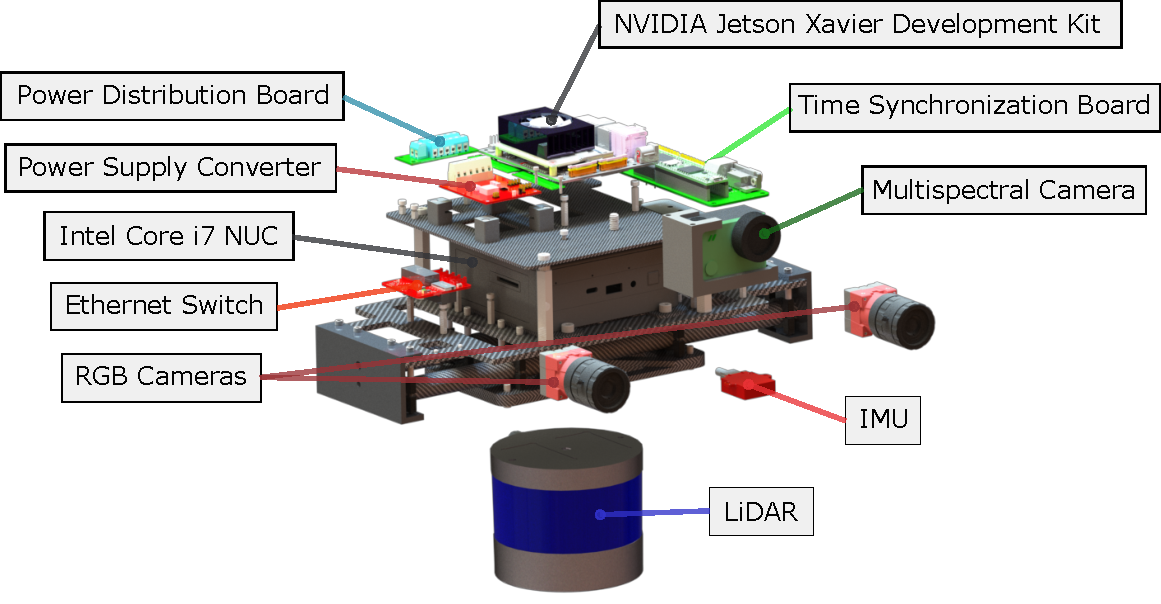
\includegraphics[width=0.55\textwidth]{figs/methods/datasets/payload_annotated.pdf}
    \hfill
    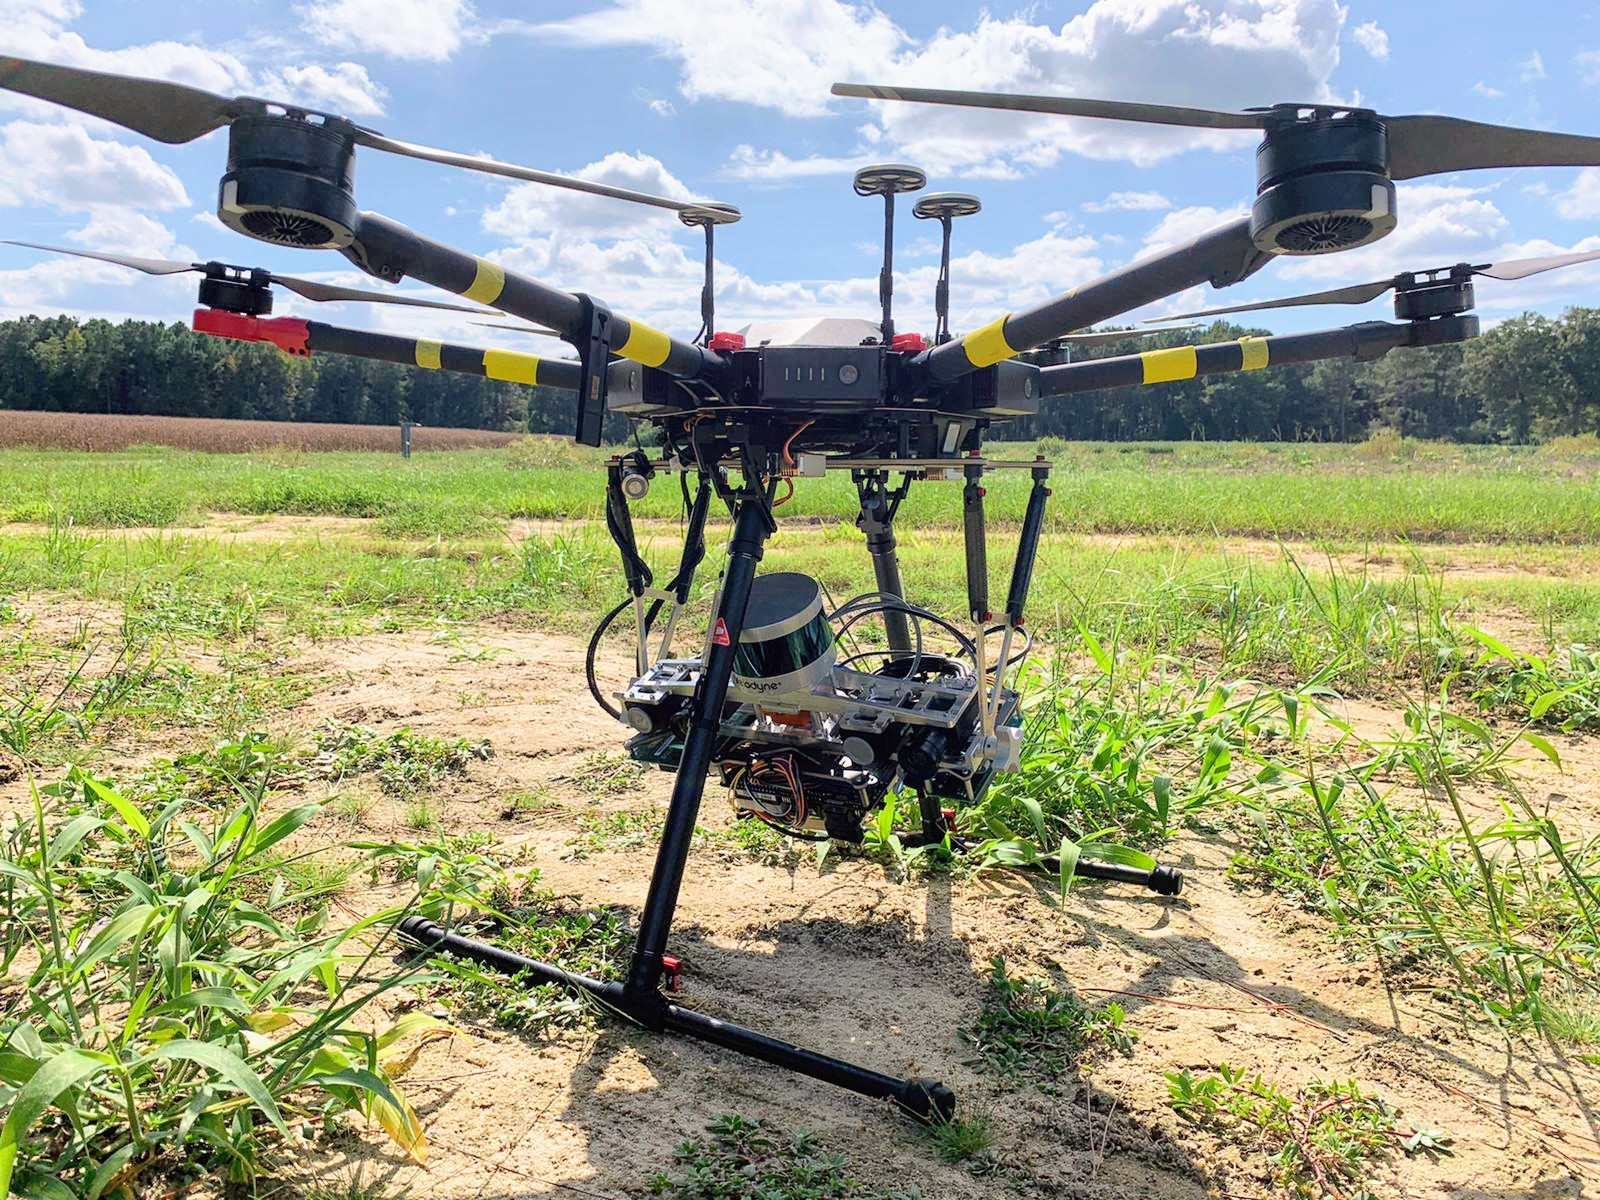
\includegraphics[width=0.37\textwidth]{figs/methods/datasets/payload_on_drone.jpeg}
    \caption{The multi-sensor payload designed by our collaborators. This was used for collecting rich forestry drone data. Photo credit to Winnie Kuang.}
    \label{fig:methods:payload}
\end{figure}

This payload is modular and could be mounted to different drones with different inclination angles. In these experiments, we used two large commercially-oriented drones, a DJI Matrice 600 and an AltaX Freefly. We flew a variety of different experiments, both under the canopy and over the canopy. In the under-canopy settings, we flew in small clearings between trees under manual control. Babak B. Chehreh from the University of Coimbra served as our pilot. In these experiments, we tried to survey the boundary of the clearing exhaustively by using an oblique payload orientation of 30 degrees from horizontal.

In the over canopy setting, we used a commercial flight planner. This allowed us to do a coverage plan over a region, using a traditional "lawnmower" pattern. Our altitude and overlap varied by experiment, but in most cases it was approximately 40 meters.


\begin{table}[]
\centering
\begin{tabular}{|l|l|l|l|l|}
\hline
\textbf{Name} & \textbf{Location} & \textbf{Platform} & \textbf{Environment} & \textbf{\makecell{Flight Pattern\\(camera angle \\from horizontal)}}\\
\hline
Coimbra & \makecell{Coimbra,\\ Portugal} & \makecell{Matrice 600 \\with custom payload} & \makecell{Forest path} & \makecell{Manual out \\and back (30)} \\ 
\hline
Oporto & \makecell{Oporto,\\ Portugal} & \makecell{Matrice 600 \\with custom payload} & \makecell{Forest clearing\\ with grass} & \makecell{Manual observations\\ of the boundary (30)}\\
\hline
Gascola & \makecell{Pittsburgh,\\ PA USA} & \makecell{Freefly with \\custom payload} & \makecell{Trees, shrubs,\\ and grasses} & \makecell{Lawnmower \\ over canopy\\ (75)} \\
\hline
Wharton & \makecell{Hammonton,\\ NJ USA} & \makecell{Matrice 600 with \\custom payload} & \makecell{Forest with road} & \makecell{Manual oval \\ over canopy\\ (60)} \\
\hline
Stowe & \makecell{Stowe,\\ VT USA} & \makecell{DJI Air 2s} & \makecell{Forest} & \makecell{Lawnmower (90)} \\ 
\hline
Emerald \cite{Young2022} & \makecell{Lake Tahoe,\\ CA USA} & \makecell{DJI Mavic 2} & \makecell{Forest} & \makecell{Lawnmower (90)} \\ 
\hline
\end{tabular}
\caption{A summary of drone datasets used in this work.}
\end{table}

\subsection{Optical remote sensing data}
Optical remote sensing data is captured by sensors onboard satellites or airplanes. This class of data is extremely powerful because it enables understanding at planetary scales, often with no or low cost to the data consumer. Remote sensing data can take many forms such as LiDAR, synthetic aperture radar (SAR), and optical. In this work, we focus on optical data, since it is conceptually most similar to what we capture from drones. This data is collected by an electro-optical sensor which takes images of the earth. Then, the images are registered together and referenced into absolute geospatial coordinates. This process relies on the estimated pose of the platform when the image was taken, the height of the ground, and manual corrections. From there, an orthographic render is generated. This is a projection of the data into a top-down view, which is commonly aligned with the axes of geospatial coordinate system used to define the location. Many satellite data sources capture bands outside of the visible wavelength. Sensors which capture a x to y number of bands are termed multi-spectral and sensors which captured y to z bands are termed hyper-spectral. In this work, we focus primarily on data collected by the National Aerial Imagery Program (NAIP) multi-spectral data source which contains red, blue, green and near-infrared bands. This data is collected at an interval of at most every three years over the continental US. It is obtained using aircraft, which are generally contracted specifically for this purpose. The resolution per pixel is 0.6 meters, which means that it is relatively high for a free data product with a significant extent.

\begin{figure}
    \centering
    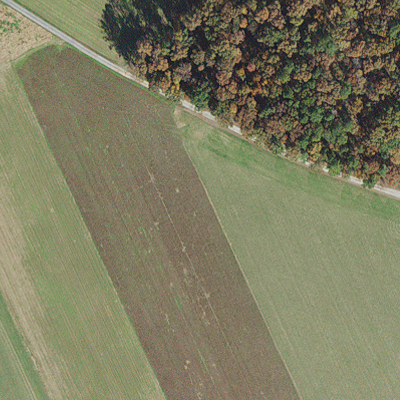
\includegraphics[width=0.5\textwidth]{figs/methods/datasets/NAIP_example.png}
    \caption{An example NAIP image crop.}
    \label{fig:methods:NAIP_example}
\end{figure}





\section{Geometric understanding of forests using drone data}
\subsection{Photogrametry}
\begin{itemize}
    \item TODO We used Agisoft  
    \item TODO The images are initialized with the GPS coordinates
\end{itemize}

\subsection{SLAM}    
Since SLAM is not the focus of this work, we choose to use results from our collaborators on these datasets. They tuned LIO-SAM\cite{Shan2020LIO-SAM:Mapping} to work well in this environment.
\begin{itemize}
    \item TODO expand 
\end{itemize}


\section{Semantic mapping for forests}
\subsection{Semantic segmentation}
In the image domain, we use a segmentation network based on a transformer architecture called SegFormer \cite{Xie2021}. Given the relatively low amount of real-world images in our training dataset, this network was especially suitable since it showed strong performance on benchmark datasets and good generalization capabilities. We trained this model using the default parameters used in the MMSegmentation \cite{MMSegmentation} implementation. 

We only labeled data coarsely because it was shown to be effective in \cite{Davila2022ADAPT:AI}. We used the VIAME toolkit 
    
\begin{figure}
    \centering
    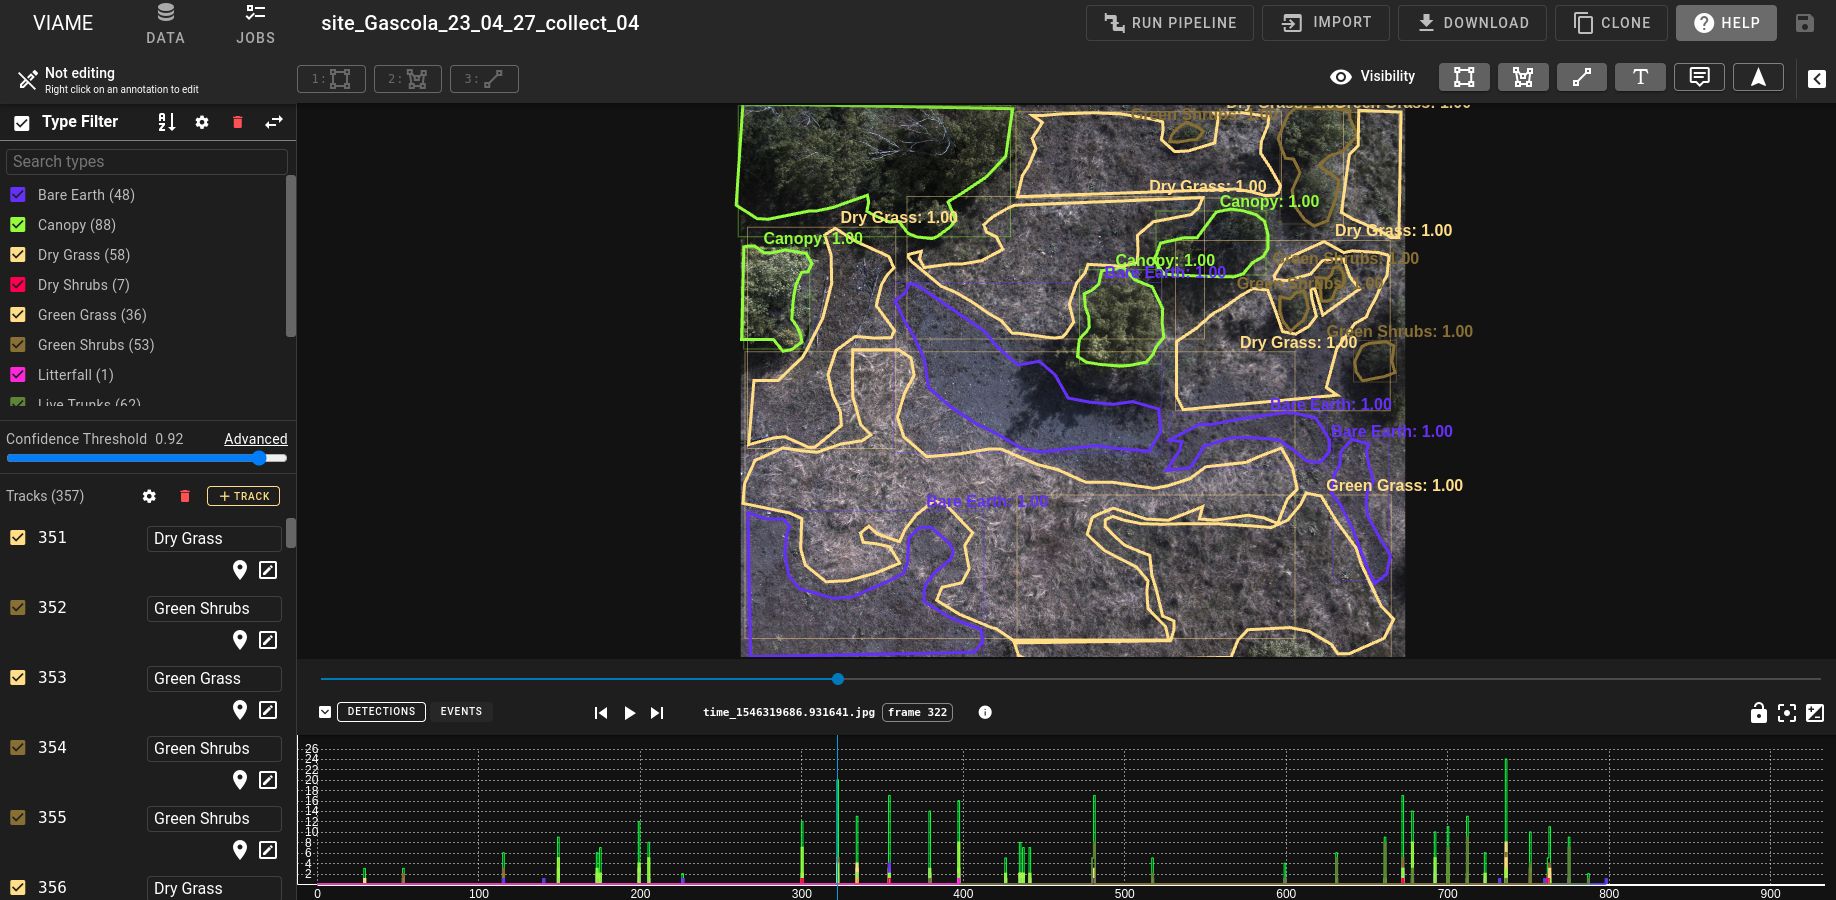
\includegraphics[width=\textwidth]{figs/methods/semantic_mapping/viame_example.png}
    \caption{Example manual annotations using the VIAME toolkit, a free and open source web annotator with potential support for integrated model training.}
    \label{fig:methods:manual-annotations}
\end{figure}


\subsection{LiDAR camera work}

\begin{figure}
    \centering
    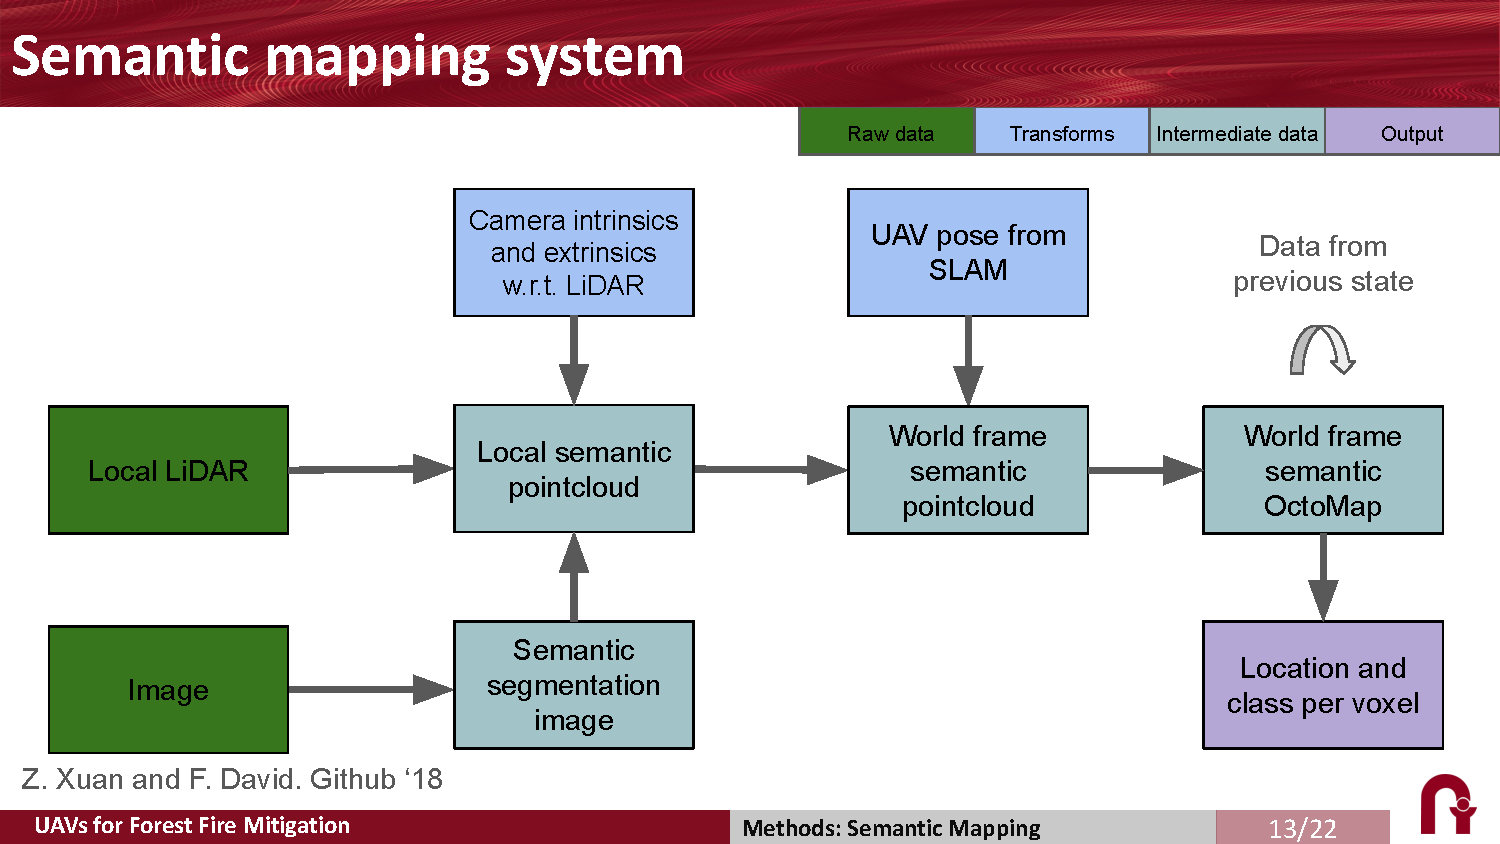
\includegraphics[width=\textwidth, clip, trim={0 1.5cm 0 1.8cm}]{figs/methods/semantic_mapping/semantic_mapping_overview.pdf}
    \caption{An overview of the LiDAR-camera semantic mapping system}
    \label{fig:lidar-camera-semantic-mapping}
\end{figure}

Subsequently, we modified an approach for RGB-D semantic SLAM \cite{semantic_slam} to project the detections from the image to the LiDAR domain (i.e., three-dimensional). First, the image is passed through the semantic segmentation network to get a classification result for each pixel. Using the extrinsics of the LiDAR relative to the camera, we transformed the LiDAR measurements into the camera's coordinate frame. Then, using the calibrated camera intrinsic, we project each LiDAR point into the image plane. Points within the field of view of the camera are assigned a classification label from the corresponding pixel in the semantic map. This semantically-textured point cloud is transformed into the inertial reference frame using the current pose of the drone estimated by our SLAM system. 

We use an octomap \cite{hornung13auro} representation to efficiently discretize the generated semantic point cloud into voxels. Each voxel has a resolution of 0.05m and contains information about the predicted classification. Each time a new semantic point cloud is created, it is used to update this global octomap. Since each voxel can contain multiple observations, we use two approaches to determine the aggregate classification. The first method assigns the class label using the highest-confidence prediction from the neural network that corresponds to that voxel. Alternatively, we use a Bayesian method which maintains a probability distribution over the classes. Each new observation is multiplied by the current distribution and then re-normalized. The voxel is then labeled with the most probable class.

%\subsection{Adding semantics to meshes}
%\begin{itemize}
%    \item The semantics are predicted for each image
%    \item The semantics are predicted onto the mesh faces
%    \item They are aggregated across the different viewpoints using...
%
%\begin{figure}
%    \centering
%    \includegraphics{example-image-a}
%    \caption{Single-view semantic prediction}
%    \label{fig:single-view-semantic-pred}
%\end{figure}
%
%\end{itemize}

\section{Tree detection in top-down data}
The goal of this work is to study tree detection at multiple scales, given a realistic set of operational constraints. Specifically, we assume that we have easy access to aerial or satellite data covering a broad region. This data is assumed to be at the lowest spatial resolution. Within this region, we have a drone survey which covers a smaller spatial extent but is at a higher resolution. Finally, we have an even smaller region where we know the location and extent of every tree. This could either be from field reference data or manual annotation of the drone orthomosaic. Our goal is to accurately detect the trees in the entire region of interest that's covered by the satellite data. 

\begin{figure}
    \centering
    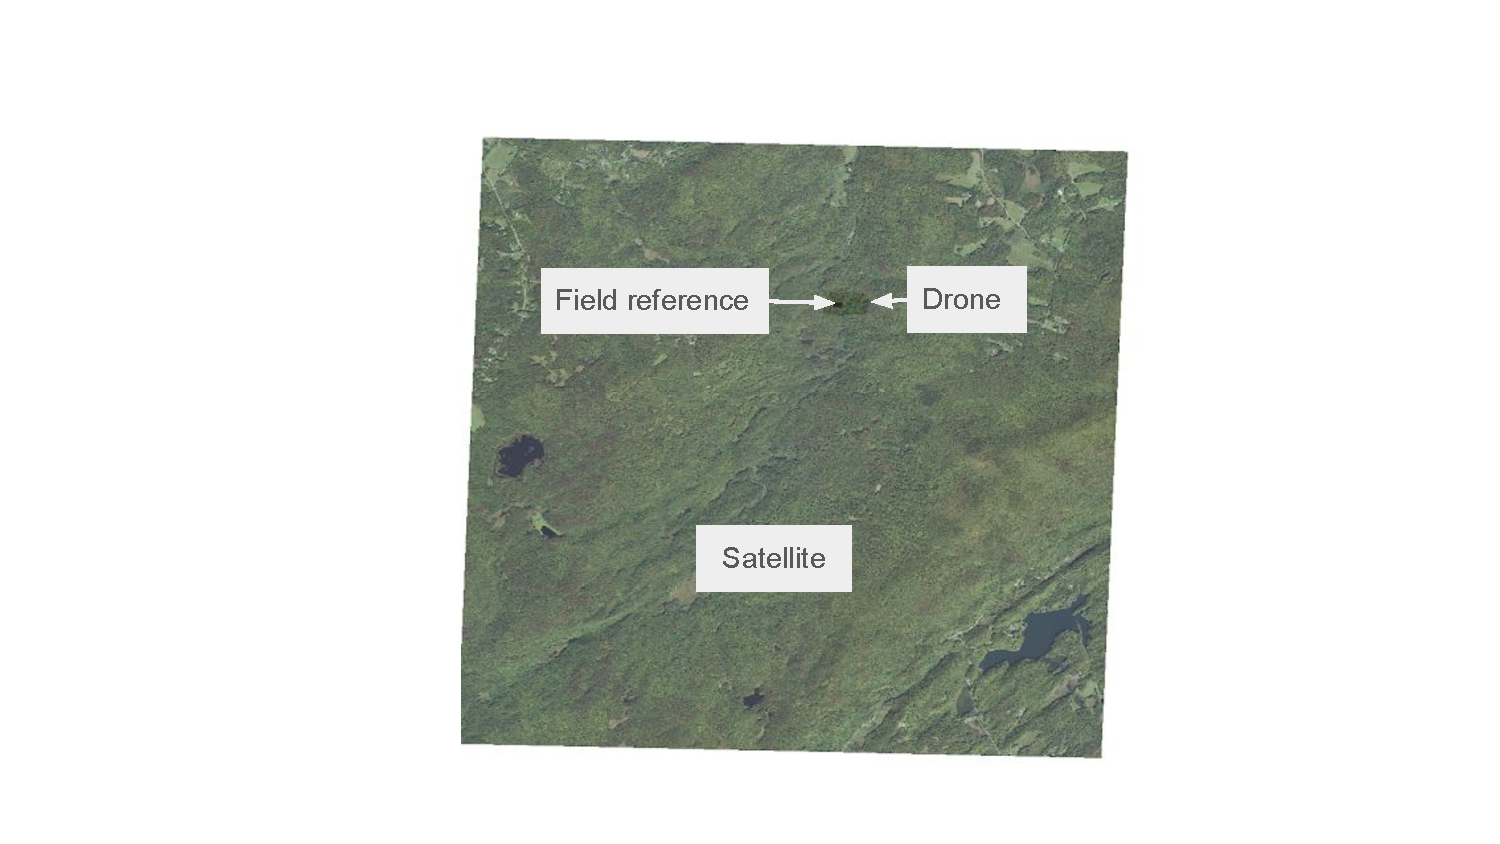
\includegraphics[width=0.7\textwidth, trim={6cm 0cm 5cm 1cm},clip]{figs/methods/tree_detection/multi_scale_data.pdf}
    \caption{Multiple scales of tree detection data}
    \label{fig:enter-label}
\end{figure}

In this section, we explore tree detection based solely on GPS-tagged images from a commodity drone survey. We use a fairly common workflow which involves first building a 3D model of the scene, then rendering an orthomosaic, and finally generating predictions on the orthomosaic using a deep convolutional object detector. Specifically, we use the same Agisoft Metashape parameters as described in previous sections. We generate an orthomoasiac using the default settings, which leverages a mosaicing approach to generating the texture and blends the observations based on the mesh geometry. We then use DeepForest \cite{Weinstein2020DeepForest:Delineation}, which is a deep learning model trained on a diverse set of trees labeled in drone orthomosaics, to predict the bounding boxes for each tree in the image. An important consideration when using DeepForest is the geospatial input resolution, because this is known to have a strong impact on performance. Since our orthomoasics are in geospatial coordinates, we know the resolution in meters per pixel. Therefore, we resample the images to a consisent resolution of 0.1 meters per pixel, which matches the data that DeepForest was trained on.

To serve as training and test data, we manually labeled a small region of trees. 

\begin{figure}
    \subfloat{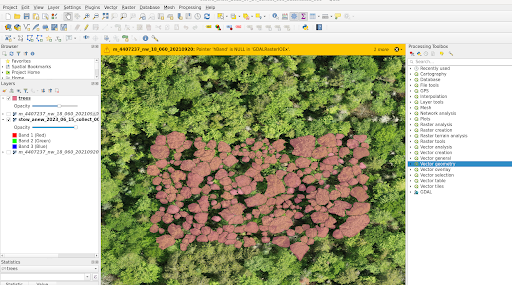
\includegraphics[width=0.45\textwidth, trim={4cm 0cm 3.5cm 2cm}, clip]{figs/methods/tree_detection/annotations.png}}
    \hfill
    \subfloat{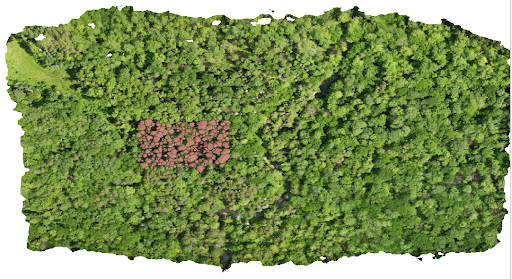
\includegraphics[width=0.45\textwidth]{figs/methods/tree_detection/annotations_scale.png}}
    \caption{Caption}
    \label{fig:enter-label}
\end{figure}

To conduct meaningful experiments with multiple types of geospatial data, it is important to have accurate registration. 

\begin{itemize}
    \item TODO finish talking about the experimental setup 
\end{itemize}


\section{Informative path planning}

Since we have developed drone monitoring systems and shown how these observations can be extrapolated to a larger scale with satellite data, a natural question is where to collect observations with the drone. There are several factors we must take into account determining a sampling strategy. The first consideration is that drones have a finite battery life which governs the distance they can cover. Secondly, commodity drones require that their entire flight plan be specified before takeoff, and they do not provide functionality to implement re-planning strategies in flight. Thirdly, we make some simplifying assumptions to define the type of observations we take. Specifically, we assume that the atomic observation is a plot, or a small lawnmower survey of a fixed square size. We further assume that the user specifies a fixed number of plots to visit. Since it will take a fixed amount of time to execute the plot surveys, the maximum available time to traverse between plots is the maximum time of a full flight minus the time taken to complete the surveys. The algorithm's decision variables are where to place these plots and in what order to visit them, subject to the maximum time available to traverse between them.

In optimization problems, it is important to define a clear metric for desirable outcomes. The goal of our work is to collect samples that...
\begin{itemize}
    \item Talk about how we want these samples to be informative about the rest of the region 
\end{itemize}


\subsection{Feature extraction on remote sensing data}
We begin by running MOSIAKS \cite{Rolf2021}. Then we do dimensionality reduction with PCA or a VAE. This was motivated by the work of \cite{Candela2020PlanetaryMapping}. Then features are unitized. 

In this work, we need a system that can generate predictions from aerial/satellite data when trained on in-situ measurements such as species classification or biomass. Many domain-specific models exist for these tasks for a given modality. However, it is challenging to find or implement these models, especially for a non-technical domain expert. 

As we continued to work on this project, and guided by the report feedback, we realized the value of a prediction system that is explicitly designed to work with very few training samples. This is specifically helpful if we want to collect a single set of labels and then train a preliminary model to inform the next round of sampling. While there are many approaches from the field of low-shot learning, they are often complex and tailored to a specific task and domain. To reduce the complexity of our approach and try to develop a generalizable method, we leverage Gaussian Processes (GPs) \cite{Rasmussen2004} implemented in \texttt{GPytorch}\footnote{\url{https://gpytorch.ai/}}. This prediction system is common in many related works because it provides an explicit uncertainty, which can be used to inform sampling, along with the prediction. While GPs are often used for regression tasks, extensions exist for classification, such as \cite{milios2018dirichletbased}, which is implemented in \texttt{GPytorch}.

One major limitation of GPs is they are best suited to problems with several dozen features or fewer. Therefore, we must design a feature engineering strategy that produces useful features for these GPs to learn over. Directly using the channels of each satellite pixel does not capture the textures of the scene, which are important for moderately-high resolution data. While CNNs are commonly used for feature extraction, there is not the same diversity of pretrained models for satellite data as there are for other forms of imagery common in the computer vision community. However, recent work has shown than semi-random features are a strong alternative to even task-specific CNN features \cite{Rolf2021}. Specifically, this work proposes MOSAIKS, which are features computed by convolving random cropped patches of the image across the entire archive of satellite data. As shown in this work, these features are useful for a variety of downstream tasks. However, since the dimensionality of the feature vector is often in the hundreds or thousands (corresponding to the same number of randomly-sampled patches) it's too large to be used as an input to a GP. Therefore, we apply dimensionality reduction by using PCA to reduce the features down a reasonable number. In this case, we use 6. An example of this feature extraction method can be seen in Figure \ref{fig:unsupervised} and Figure \ref{fig:TSNE} shows that the features appear to separate nicely based on class.


    
\subsection{Gaussian Proccess uncertainty modeling}
\begin{itemize}
    \item Many works try to minimize the entropy of a Gaussian Proccess. This tool is especially nice because GPs can generate uncertainty predictions by only observing the features of a set of samples and not the labels.
\end{itemize}
\subsection{Remote-sensing Aware Planning Through Observation Randomized Sampling (RAPTORS)
}
\begin{figure}
    \centering
    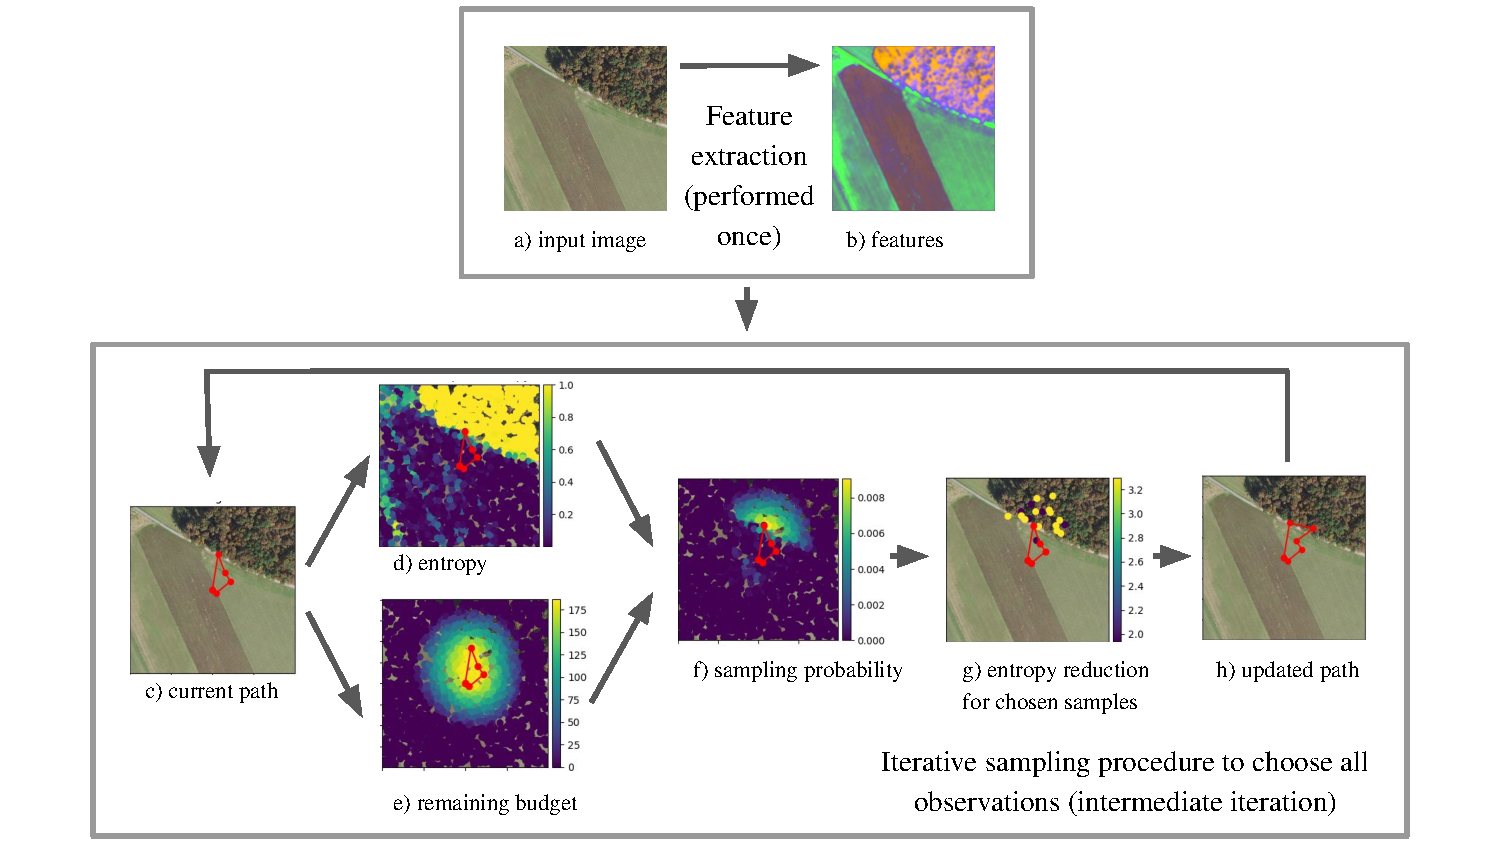
\includegraphics[width=\textwidth, clip, trim={1.5cm, 0, 1.5cm, 0}]{figs/methods/IPP/RAPTORS_concept_figure.pdf}
    \caption{This figure describes the workflow of a generalizable long-horizon path planner for selecting a set of drone observations. The required inputs are a satellite tile a), the drone's starting location, the path length budget, and the number of samples. Descriptive features are extracted from the image using random patches from the image as convolutional kernels, following the MOSAIKS method, and then compressed with PCA b). A full path is then built iteratively offline. At each iteration, the current path is provided as input, as shown in c). Then the uncertainty for a set of candidate locations is computed using a Gaussian Process d) and the remaining flight budget taking into account the current path is computed e). Then the uncertainty and remaining budget are multiplied and normalized to obtain a probability of evaluating each sample further. A set of samples are selected and the entropy reduction is calculated if each one were added to the Gaussian Process model f). Then the best sample is added and the path ordering is recomputed using a traveling salesman solver g). Then the process is repeated to plan the next observation until the requested number of observations are planned for. Only then is the path executed by the drone.
}
    \label{fig:methods:IPP_raptors_overview}
\end{figure}

\begin{algorithm}
\caption{RAPTORS}\label{alg:methods:RAPTORS}
\begin{algorithmic}
\State $F = extract\_features(I)$
\end{algorithmic}
\end{algorithm}

\begin{algorithm}
\caption{extract\_features}\label{alg:methods:extract_features}
\begin{algorithmic}
\State $F = extract\_features(I)$
\end{algorithmic}
\end{algorithm}

\begin{algorithm}
\caption{choose\_next\_sample}\label{alg:methods:choose_next_sample}
\begin{algorithmic}
\State $F = extract\_features(I)$
\end{algorithmic}
\end{algorithm}



\begin{itemize}
    \item We employ a sampling-based strategy to build a long horizon offline path. This takes in an initial location, a number of samples, and a traversal budget. The algorithm begins by computing the gaussian process uncertainty after only observing the first location. Then, a feasible region is computed using a fraction of the remaining budget. A fixed number of samples are drawn from this feasible region, using a weighted sampling based on their uncertainty. The sample which reduces the total map unceratinty the most is added to the plan. Then the points are ordered using a TSP solver. The feasible region is recomputed using the added points and the fraction of the remaining budget.
\end{itemize}